% !TeX root = ../main.tex

\chapter{}
\section{电子回旋辐射公式推导}
\label{sec:A1}
为方便研究单电子回旋运动又不失一般性,以磁场所在方向建立z轴,研究波矢沿xz所在平面的电磁波,根据电动力学,电子沿任意轨道运动时辐射电场和磁场满足方程\footnote{注:本节主要参考俞老师等离子体诊断讲义,补充了部分推导过程}
\begin{figure}[ht]
\centering
\includegraphics[width=12cm]{image50.png}
\caption{\label{fig:elecorb2}均匀磁场中电子螺旋运动图}
\end{figure}

\begin{align}
E({R}, t) & = \frac{e}{4 \pi \epsilon_{0} c R^{\prime}}\left\{\frac{\hat{q} \times[(\hat{q}-\vec{\beta}) \times \dot{\vec{\beta}}]}{(1-\hat{q} \cdot \vec{\beta})^{3}}\right\}_{\mathrm{t}^{\prime}} \\
B({R}, t) & = \frac{1}{c} \hat{q} \times \vec{E}(\mathrm{R}, \mathrm{t})
\end{align}
其中: $ t^{\prime}=t-\frac{R^{\prime}}{c}=t-\frac{\left|\vec{R}-\vec{r}\left(t^{\prime}\right)\right|}{{c}} \cong t-\frac{R}{c}+\frac{\hat{q} \cdot \vec{r}\left(t^{\prime}\right)}{c} $, 观测位置在时刻  $\mathrm{t} $ 的电场是粒子 在时刻 $ \mathrm{t}^{\prime}  $激发的, 该时刻粒子处于 $ \mathrm{r}\left(\mathrm{t}^{\prime}\right) $ 点上辐射电场频谱为:
\begin{equation}
E({R},\omega)=\frac{e}{4 \pi \epsilon_{0} c R^{\prime}} \int d t e^{-i \omega t}\left\{\frac{\hat{q} \times[(\hat{q}-\vec{\beta}) \times \dot{\vec{\beta}}]}{(1-\hat{q}\cdot \vec{\beta})^{3}}\right\}_{\mathrm{t}^{\prime}}
\end{equation}
为了方便后续计算,将时间t表示为$t'$的函数得到:
\begin{equation}\label{eq:A4}
E({R}, \omega)=\frac{e}{4 \pi \epsilon_{0} c R^{\prime}} \int d t^{\prime}\exp\left\{-i 
\omega\left(t^{\prime}+\frac{R}{c}-\frac{\hat{q} \cdot \vec{r}}{c}\right)\right\}\left\{\frac{\hat{q} 
\times[(\hat{q}-\vec{\beta}) \times \dot{\vec{\beta}}]}{(1-\hat{q} \cdot \vec{\beta})^{2}}\right\}
_{\mathrm{t}^{\prime}}
\end{equation}
利用恒等式:
\begin{equation}
\left\{\frac{\hat{q} \times[(\hat{q}-\vec{\beta}) \times \dot{\vec{\beta}}]}{(1-\hat{q}\cdot \vec{\beta})^{2}}\right\}_{\mathrm{t}^{\prime}}=\frac{d}{d t^{\prime}}\left\{\frac{\hat{q}\times(\hat{q} \times \vec{\beta})}{(1-\hat{q} \cdot \vec{\beta})}\right\}
\end{equation}
对方程\autoref{eq:A4}分步积分得
\begin{equation}\label{eq:intER}
{E}({R}, \omega)=\frac{i \omega e}{4 \pi \epsilon_{0} c R^{\prime}} \int d t^{\prime}\hat{q} \times(\hat{q} \times \vec{\beta}) e^{-i \omega\left(t^{\prime}+\frac{R}{c}-\frac{\hat{q}\cdot \vec{r}}{c}\right)}
\end{equation}
根据Parseval定理,单位立体角内辐射能量为:
\begin{equation}\label{eq:dWdw}
\frac{d^{2} W}{d \omega d \Omega}=\frac{c \epsilon_{0} R^{\prime 2}}{2 \pi}|{E}(R, \omega)|^{2}
\end{equation}
当电子辐射功远小于其动能时,电子运动轨道可忽略辐射对其自身的影响.在均匀磁场中电子的运动方程可表示为:
\begin{equation}
\frac{d}{d t}\left(\frac{m {\vv}}{\sqrt{1-\beta^{2}}}\right)=-e\left({\vv} \times {\vB_{0}}\right)
\end{equation}
其运动方程的解为
\begin{subequations}\label{eq:fmov}
\begin{align}
{\v\beta}&=\beta_\perp \left (\vec x \cos \omega_{ce}t+\vec y \sin\omega_{ce}t\right)+\beta_\parallel\vec z\\
\frac{{\vr}}{c}&=\frac{\beta_{\perp}}{\omega_{c e}}\left(\vec{x} \sin \omega_{c e} t^{\prime}-\vec{y} \cos \omega_{c e} t^{\prime}\right)+\beta_{\|} t^{\prime} \vec{z}
\end{align}
其中$\omega_{ce}=\frac{eB}{\gamma m_e}$,$\gamma=\frac{1}{\sqrt{1-\beta^2}}$
\end{subequations}
在观测位置处 ,辐射传播矢量为
\begin{equation}\label{eq:vecq}
\hat{q}=\vec{x} \sin \theta+\vec{z} \cos \theta
\end{equation}
根据\autoref{eq:fmov}和\autoref{eq:vecq},相位因子可写为:
\begin{equation}
e^{-i \omega\left(t^{\prime}-\frac{\hat{q} \cdot {\vr}}{c}\right)}=\exp \left\{-i \omega\left[t^{\prime}-\frac{\beta_{\perp}}{\omega_{c e}} \sin \theta \sin \omega_{c e} t^{\prime}-\beta_{\|} t^{\prime} \cos \theta\right]\right\}
\end{equation}
辐射偏振矢量为:
\begin{equation}
\begin{aligned}
\hat{q} \times(\hat{q} \times \vec{\beta})= & \vec{x}\left(\beta_{\|} \sin \theta \cos \theta-\beta_{\perp} \cos ^{2} \theta \cos \omega_{c e} t^{\prime}\right)-\\&\vec{y} \beta_{\perp} \sin \omega_{c e} t^{\prime} +\\&\vec{z}\left(-\beta_{\|} \sin ^{2} \theta+\beta_{\perp} \sin \theta \cos \theta \cos \omega_{c e} t^{\prime}\right)
\end{aligned}
\end{equation}
利用恒等式:
\begin{equation}
\begin{aligned}
e^{i \xi \sin \phi}&=\sum_{m=-\infty}^{+\infty} e^{i m \phi} J_{m}(\xi) \\
i \sin \phi e^{i \xi \sin \phi}&=\sum_{m=-\infty}^{+\infty} e^{i m \phi} J_{m}^{\prime}(\xi)\\
i \xi \cos \phi e^{i \xi \sin \phi}&=\sum_{m=-\infty}^{+\infty} i m e^{i m \phi} J_{m}^{\prime}(\xi)
\end{aligned}
\end{equation}
其中$ξ=\left(\frac{ωβ_⊥}{ω_c}\right)sinθ$,于是\autoref{eq:intER}中积分项为
\begin{small}
\begin{equation}
\begin{aligned}
\hat{q} \times(\hat{q} \times \vec{\beta})\exp\left\{-i \omega\left(t^{\prime}-\frac{\hat{q} \cdot {\vr}}
{c}\right)\right\}=\sum_{m=-\infty}^{+\infty}&\left\{ \vec x\left(\v\beta_\parallel \sin \theta \cos \theta-\beta_{\perp}\cos^2\theta \frac{m}{\xi}\right)\right.J_m(\xi) \\ 
\quad &+\vec y i\beta_\perp J_{m}^{\prime}(\xi)\\
\quad&+\vec z \left. \left(-\beta_\parallel \sin^2\theta +\beta_\perp \sin\theta \cos \theta \frac{m}{\xi}\right)J_m(\xi)\right\}\\
\quad&\times\exp\left\{-i \omega\left(1-\beta_\parallel \cos\theta \right)t'+im \omega_{ce}t'\right\}
\end{aligned}
\end{equation}
\end{small}
考虑共振条件$\omega(1-\beta_\parallel \cos(\theta)=m\omega_{ce}$,因此\autoref{eq:intER}为
\begin{equation}\label{eq:ERw}
\begin{aligned}
{E}(R, \omega)=&\frac{i e \omega}{2 \epsilon_{0} c R^{\prime}} \sum_{-\infty}^{+\infty} \delta\left[\left(1-\beta_{\|} \cos \theta\right) \omega-m \omega_{c e}\right]\times\\
&\left\{\vec x \left[-\frac{\cos \theta}{\sin \theta}\left(\cos \theta-\beta_{\|}\right) J_{m}(\xi)\right ] \right.+\\
&\left. \vec y i\beta_\perp J_{m}^{\prime}(\xi)+\vec z\left(\cos \theta-\beta_\parallel\right)J_m(\xi)\right\}
\end{aligned}
\end{equation}
这里利用了$\delta$函数的定义
\begin{equation}
\delta\left[\left(1-\beta_{\|} \cos \theta\right) \omega-m \omega_{c e}\right]=\frac{1}{2 \pi} \int\limits_{-\infty}^{+\infty} \exp \left(-\left[\left(1-\beta_{\|} \cos \theta\right) \omega-m \omega_{c e}\right] t^{\prime}\right) d t^{\prime}
\end{equation}
联立\autoref{eq:dWdw}和\autoref{eq:intER}得
\begin{equation}\label{eq:dWdw2}
\frac{d^{2} W}{d w d \Omega} = \frac{e^{2} \omega^{2}}{4 \pi \varepsilon_{0} c} \sum_{1}^{\infty}\left|\begin{array}{c}-\vec{{x}} \frac{\cos \theta}{\sin \theta}\left(\cos \theta-\beta_{\|}\right) J_{m}(\xi) \\-\vec{y} j \beta_{\perp} \frac{d J_{m}(\xi)}{d \xi} \\\vec{\mathrm{z}}\left(\cos \theta-\beta_{\|}\right) J_{m}(\xi)\end{array}\right|^{2} \delta^{2}\left[\left(1-\beta_{\|} \cos \theta\right) \omega-m \omega_{ce}\right]
\end{equation}
其中关于$δ^2 [(1-β_∥  cos(θ)ω-mω_{ce}]$部分可作如下处理:\par

根据卷积性质,两函数卷积的傅里叶变换等价于两函数傅里叶变换的点积
\begin{equation}
F(\omega) \cdot G(\omega)=\frac{1}{4 \pi^{2}} \int\limits_{-\infty}^{+\infty}\int\limits_{-\infty}^{+\infty} f(t) g\left(t^{\prime}-t\right)d t \exp (-i \omega t) d t^{\prime}
\end{equation}
考虑积分时间为$[-T/2,T/2]$,则
\begin{equation}\label{eq:delta2}
\delta^{2}\left(\omega^{\prime}\right)=\frac{1}{4 \pi^{2}} \int\limits_{-\frac{T}{2}}^{\frac{T}{2}}\int\limits_{-\frac{T}{2}}^{\frac{T}{2}} 1 * 1 d t \exp \left(-i \omega t^{\prime}\right) d t^{\prime}=\frac{T}{2 \pi} \delta\left(\omega^{\prime}\right)
\end{equation}
将\autoref{eq:delta2}代入\autoref{eq:dWdw2}得到总辐射强度为
\begin{equation}
\frac{d^{2} W}{d \omega d \Omega}=\frac{T e^{2} \omega^{2}}{8 \pi^{2} \epsilon_{0} c} \sum_{1}^{\infty}\left[\left(\frac{\cos \theta-\beta_{\|}}{\sin \theta}\right)^{2} J_{m}^{2}(\xi)+\beta_{\perp}^{2} J_{m}^{\prime 2}(\xi)\right] \delta\left[\left(1-\beta_{\|} \cos \theta\right) \omega-m \omega_{c e}\right]
\end{equation}
辐射功率P可表示为W除以总辐射时间T,最终得到单电子单位频率单位立体角内总辐射功率为:
\begin{equation}
\frac{d^{2} P}{d \omega d \Omega}=\frac{e^{2} \omega^{2}}{8 \pi^{2} \epsilon_{0} c} \sum_{m=1}^{\infty}\left[\left(\frac{\cos \theta-\beta_{\|}}{\sin \theta}\right)^{2} J_{m}^{2}(\xi)+\beta_{\perp}^{2} J_{m}^{\prime 2}(\xi)\right] \delta\left[\left(1-\beta_{\|} \cos \theta\right)\omega-m \omega_{c e}\right]
\end{equation}
其中X波对应的偏振方向为$\hat{y}$,其相应的辐射功率为
\begin{equation}\label{eq:Xradiation}
\frac{d^{2} P}{d \omega d \Omega}=\frac{e^{2} \omega^{2}}{8 \pi^{2} \epsilon_{0} c} \sum_{m=1}^{\infty}\left[\beta_{\perp}^{2} J_{m}^{\prime 2}(\xi)\right] \delta\left[\left(1-\beta_{\|} \cos \theta\right)\omega-m \omega_{c e}\right]
\end{equation}





\section{吸收系数方程坐标变换}\label{sec:A2}
由于实际计算中采用$(ξ,p)$坐标系,将辐射吸收\autoref{eq:alpha2}中$p_∥$、$ϵ$分别通过$m_e c$以及$m_e c^2$无量纲化,并对速度分布函数f采用归一化函数得:
\begin{equation}
\alpha_{\omega}=-\frac{8 \pi^{3} c^{2}n_0}{m_{e} c^{2} \omega^{2}} \int \eta_{1}^{i}\left({\vp}^{\prime}\right) *\left[\frac{\partial f}{\partial p_{\|}} * \cos \theta+\frac{\partial f}{\partial \epsilon}\right] d {\vp}^{\prime}
\end{equation}
根据
\begin{equation}
\begin{aligned}
p_{\|} & =p \cdot \xi  \\
\epsilon & =\sqrt{1+p^{2}}
\end{aligned}
\end{equation}
可得
\begin{equation}
\begin{array}{l}
p=\sqrt{\epsilon^{2}-1} \\
\xi=\frac{p_{\|}}{\sqrt{\epsilon^{2}-1}}
\end{array}
\end{equation}
又因为
\begin{align}
\frac{\partial f}{\partial p_{\|}} & = \frac{\partial f}{\partial p} \frac{\partial p}{\partial p_{\|}}+\frac{\partial f}{\partial \xi} \frac{\partial \xi}{\partial p_{\|}} \\
\frac{\partial f}{\partial \epsilon} & = \frac{\partial f}{\partial p} \frac{\partial p}{\partial \epsilon}+\frac{\partial f}{\partial \xi} \frac{\partial \xi}{\partial \epsilon} 
\end{align}
根据:
\begin{equation}
\begin{aligned}\frac{\partial p}{\partial p_{\|}} & =0 \\\frac{\partial p}{\partial \epsilon} & =\frac{\epsilon}{\sqrt{\epsilon^{2}-1}}=\frac{\sqrt{1+p^{2}}}{p} \\\frac{\partial \xi}{\partial p_{\|}} & =\frac{1}{\sqrt{\epsilon^{2}-1}}=\frac{1}{p} \\\frac{\partial \xi}{\partial \epsilon} & =\frac{-\epsilon p_{\|}}{\left(\epsilon^{2}-1\right)^{\frac{3}{2}}}=-\frac{\xi \sqrt{1+p^{2}}}{p^{2}}\end{aligned}
\end{equation}
最终可得:
\begin{align}
\frac{\partial f}{\partial p_{\|}} & = \frac{\partial f}{\partial p} \frac{\partial p}{\partial p_{\|}}+\frac{\partial f}{\partial \xi} \frac{\partial \xi}{\partial p_{\|}}  = \frac{1}{p} \frac{\partial f}{\partial \xi} \\
\frac{\partial f}{\partial \epsilon} & = \frac{\partial f}{\partial p} \frac{\partial p}{\partial \epsilon}+\frac{\partial f}{\partial \xi} \frac{\partial \xi}{\partial \epsilon}  = \frac{\sqrt{1+p^{2}}}{p} \frac{\partial f}{\partial p}-\frac{\xi \sqrt{1+p^{2}}}{p^{2}} \frac{\partial f}{\partial \xi}
\end{align}
于是吸收系数计算方程化为
\begin{equation}
\alpha_{\omega}=-\frac{8 \pi^{3} c^{2}n_0}{m_{e} c^{2} \omega^{2}} \int \eta_{1}^{i}(\beta, \xi)\left[\frac{1}{p} \frac{\partial f}{\partial \xi} \cos \theta+\frac{\sqrt{1+p^{2}}}{p} \frac{\partial f}{\partial p}-\frac{\xi \sqrt{1+p^{2}}}{p^{2}} \frac{\partial f}{\partial \xi}\right] 2 \pi p^{2}d p d \xi
\end{equation}
\section{二维狄拉克函数积分}\label{sec:A3}

通过换元,狄拉克函数的二维积分可写为如下形式:
\begin{equation}
\int \delta(\mathrm{f}(\mathrm{x}, \mathrm{y})) g(\mathrm{x}, \mathrm{y}) \mathrm{dxdy}=\int \delta(\mathrm{f}) g(\mathrm{x}, \mathrm{y})\left|\frac{\partial(\mathrm{x}, \mathrm{y})}{\partial(\mathrm{u}, \mathrm{v})}\right| \mathrm{dudv}
\end{equation}
 
 其中u,v为任意两族曲线,取u为f(x,y),v为x,则
\begin{equation}
\begin{aligned}
\left|\frac{\partial(\mathrm{x}, \mathrm{y})}{\partial(\mathrm{u}, \mathrm{v})}\right|=&\left|\frac{\partial(\mathrm{x}, \mathrm{y})}{\partial(\mathrm{f}, \mathrm{x})}\right|\\
=&\left|\begin{array}{ll}\frac{\partial x}{\partial f} & 1 \\\frac{\partial y}{\partial f} & 0\end{array}\right|\\
=&\left|\frac{\partial y}{\partial f}\right|=\frac{1}{\left|\frac{\partial f}{\partial y}\right|}
\end{aligned}
\end{equation}

\begin{itemize}
\item
当$f(x,y)=0$,对于任意x,只存在对应唯一解$y_i (x)$,且$∂f/∂y |_{(y_i,x)}≠0$时:
\begin{equation}
\int \delta(\mathrm{f}(\mathrm{x}, \mathrm{y})) \mathrm{g}(\mathrm{x}, \mathrm{y}) \mathrm{dxdy}=\int \frac{\mathrm{g}\left(y_{i}, \mathrm{x}\right) }{\left|\frac{\partial f}{\partial y}\right|_{y_{i}(x)}}\mathrm{dx}
\end{equation}


\item
当$f(x,y)=0$,对于任意x,存在对应多个$y_i$的解,且$∂f/∂y |_{(y_i,x)}≠0$时:
\begin{equation}
\int \delta(\mathrm{f}(\mathrm{x}, \mathrm{y})) \mathrm{g}(\mathrm{x}, \mathrm{y}) \mathrm{dxdy}=\int \sum_{i} \frac{\mathrm{~g}\left(y_{i}, \mathrm{x}\right) }{\left|\frac{\partial f}{\partial y}\right|_{y_{i}, x}} \dif x
\end{equation}
\end{itemize}
\section{射线追迹}\label{sec:A4}
在真空中由于介电常数不变,光一般是沿着直线传播,等离子体中介电常速和等离子体密度、磁场等关系密切,导致电磁波的折射率随空间不断变化,此时电磁波的传播路线取决于折射率的分布。当折射率变化量在电磁波波长范围内可以忽略不记时($|∇k|/k^2 ≪1,|∇μ|/μ^2 ≪1$,WKB近似条件)折射率由局域值决定,在满足这种几何光学近似条件下电磁波的轨迹可通过射线追迹方程描述\cite{RN1958}:
\begin{equation}
\begin{aligned}
\frac{d r}{d t}&=\frac{\partial \omega}{\partial k} \\
\frac{d k}{d t}&=-\frac{\partial \omega}{\partial r}
\end{aligned}
\end{equation}
其中r为光传播得位置,k为光得波矢,且二者之间满足关系
\begin{equation}
\omega^{2}=\frac{k^{2} c^{2}}{n^{2}}
\end{equation}
因此有
\begin{align}
\frac{\partial \omega}{\partial k} & = \frac{k c^{2}}{\omega n^{2}}\\ \frac{\partial \omega}{\partial r} & = -\frac{\omega}{2 n^{2}} \frac{\partial n^{2}}{\partial r}
\end{align}
磁化冷等离子体中,电磁波折射率n的方程满足Appleton-Hartreen公式:
\begin{equation}
n^{2}=1-\frac{X(1-X)}{1-X-\frac{1}{2} Y^{2} \sin ^{2} \theta \pm\left[\left(\frac{1}{2} Y^{2} \sin ^{2} \theta\right)^{2}+(1-X)^{2} Y^{2} \cos ^{2} \theta\right]^{\frac{1}{2}}}
\end{equation}
这里$X=ω_{pe}^2/ω^2$ ,$Y=ω_{ce}/ω,θ=acos⁡((k∙B)/|k||B| )$,当θ=0时,电磁波传播方向平行磁场。
由于电子回旋频率$ω_{ce}$以及等离子体振荡频率$ω_{pe}$和磁场等离子体密度相关,为了准确求出波在托卡马克中传播路径,我们需要获得托卡马克放电过程中密度和磁场分布。EAST托卡马克efit数据库中上传了每一炮极向磁通$ψ$信息,$ψ$包含了放电过程中极向磁面信息和极向磁场强度分布(如\autoref{fig:polarBs}(a)),考虑磁面上具有相同密度温度分布,我们可以将沿径向的一维密度分布信息延拓到整个闭合磁面以内(如\autoref{fig:polarBs}(b)),其中沿径向的密度分布可以通过point(干涉仪)诊断或自己给定,同时,我们假设等离子体参数分布具有环向对称性(没有MHD不稳定性产生),这样我们就可以获得三维空间的密度和磁场信息,然后利用插值的方法去获取电磁波传播到空间中某一个点时具有的密度和磁场。

如\autoref{fig:viewxyz}所示,在笛卡尔坐标系中我们取xz平面为参考平面,其中$x>0$的半边平面对应的环向角$α=0$。在该参考平面内,根据磁面的定义,极向面中磁场强度分别为:
\begin{align}B_{x} & = -\frac{1}{x} \frac{\partial \psi}{\partial z}\\ 
B_{z} & = \frac{1}{x} \frac{\partial \psi}{\partial x}\\
B_{y} & = B_{0} \frac{x_{0}}{x}
\end{align}
其中$x0$表示磁轴位置。该方程满足$\nabla\cdot B=0$,即:
\begin{equation}
\frac{1}{x}\frac{\partial}{\partial x}(xB_x)+\frac{\partial B_z}{\partial z}+\frac{\partial B_y}{\partial y}=0
\end{equation}
当极向面所处环向角为$α$时,对应的磁场强度分别为
\begin{align}
\left[\begin{array}{l}
B_{x}{ }^{\prime} \\
B_{y}{ }^{\prime} \\
B_{z}{ }^{\prime}
\end{array}\right] & = \left[\begin{array}{ccc}
\cos \alpha & -\sin \alpha & 0 \\
\sin \alpha & \cos \alpha & 0 \\
0 & 0 & 1
\end{array}\right]\left[\begin{array}{l}
B_{x} \\
B_{y} \\
B_{z}
\end{array}\right]
\end{align}
密度分布满足
\begin{equation}
n_{e}(r, \alpha)=n_{e}\left(r, \alpha^{\prime}\right) \text {, 其中 } r=\sqrt{x^{2}+y^{2}}
\end{equation}
这样就可以获得三维空间中磁场分布和密度分布,然后利用4阶龙格库塔方程即可求解完整的射线路径。
\begin{figure}[ht]
\centering
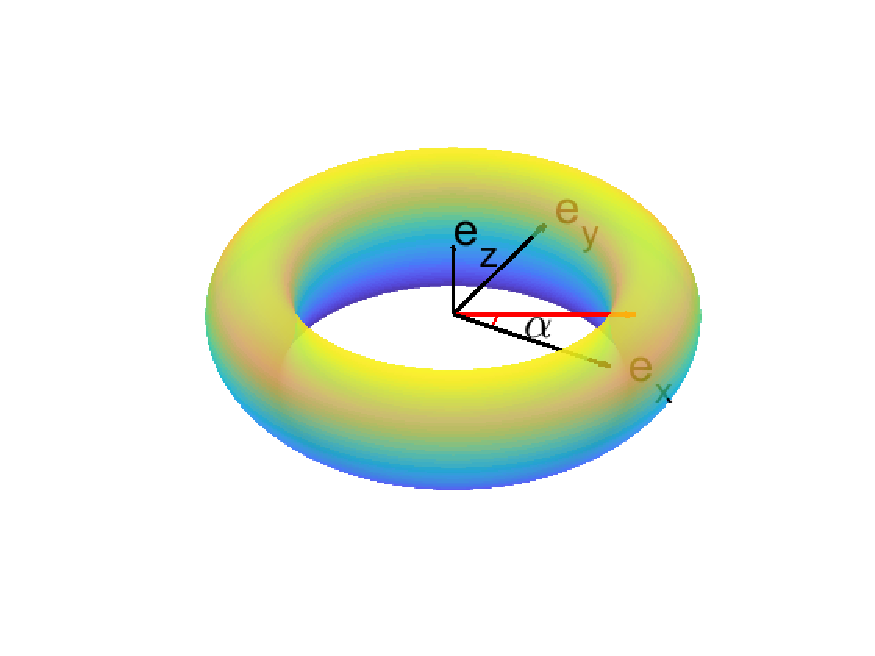
\includegraphics[width=12cm]{image117.jpeg}
\caption{\label{fig:viewxyz}定义Tokamak坐标系}
\end{figure}
\begin{figure}[ht]
\centering
\begin{overpic}[scale=0.6]{image118.png}
 \put(3, 95){$(a)$}
  \end{overpic}
\begin{overpic}[scale=0.6]{image119.png}
 \put(3,95){$(b)$}
  \end{overpic}
%\includegraphics[width=12cm]{image118.png}
\caption{\label{fig:polarBs}(a)Tokamak极向磁面分布,最外圈蓝线表示最后闭合磁面(b)Tokamak中等离子体密度空间分布}
\end{figure} \par
通过设置波的传播方向和初始位置(如\autoref{fig:3Dset}),我们就可以计算沿任意方向电磁波的传播轨迹,进而研究波在等离子体中的特征,为等离子体辐射传播提供路径信息。Ray-tracing3D代码逻辑如\autoref{alg:algorithm1}所示。

%\begin{figure}[ht]
%\centering
%\includegraphics[width=12cm]{image119.png}
%\caption{\label{fig:nedistr}Tokamak中等离子体密度空间分布}
%\end{figure}

\begin{figure}[ht]
\centering
\includegraphics[width=12cm]{image120.png}
\caption{\label{fig:3Dset}定义发射源位置和发射方向,其中$θ $表示k和z方向夹角,$ϕ $ 表示k在xy平面的投影方向和x轴负方向夹角}
\end{figure}




\begin{algorithm}[t]
	\caption{Framework of Ray-tracing3D}
	\label{alg:algorithm1}
	\KwIn{Choose the wave mode:$ \mathcal{L} \text{or} \mathcal{O}$;
Wave frequency:$\mathcal{f}\text{;}$
Toroidal Magnetic  value:$ \mathcal{B}\text{;}$\\
Wave positions:$\mathcal{\vr}\text{;}$
Flight time:$\mathcal{t}\text{;}$
Plasma density:$\mathcal{n_e}$}
	\KwOut{Figure of ray in Tokamak}  
	\BlankLine
     Download magnetic flux surface from $\mathcal{efit}$; \\
     Initialize $\mathcal{n_e}$ profile on magnetic surface;	\\
     Initialize poloidal magnetic profile;
	
	\While{\textnormal{nstep$\le$Totalsteps}}{
		Get the position of ray ;

		
		\ForEach{task in Ray-tracing3D}{
			Compute the dielectric constant at the ray poisition;
			
			Calculate the Ray-tracing equations;
			
                Update the  new ray position by Runge-Kutta 4th Order method;
		}
           nstep=nstep+1;\\
		Renew $\vr$ and $\vk$; 
	}
	
Show the trace  of ray in Tokamak

\end{algorithm}













根据EAST第104150炮第6~s磁面结构,假设芯部等离子体密度为$2\times10^{19}~/m^3$,沿半径成二次抛物线分布,磁轴处磁场强度为2~T,发射源位置处在$α=0,x=2.4~m,θ=π/2$,$ϕ=8.8^o$,y方向从-0.3~m到0.3~m依次排开6个,发射源以$f=110~Ghz$,X-mode向等离子体发射以此模拟ECEI偏离垂直磁场方向时接收光路特征,其三维视图如\autoref{fig:3Dtracing}。
\begin{figure}[ht]
\centering
\includegraphics[width=12cm]{image122.pdf}
\caption{\label{fig:3Dtracing}射线追迹三维视图}
\end{figure}
从\autoref{fig:2Dtracing}(a)中可以看出在密度为$2\times10^{19}~/m^3$,纵场为2~T的条件下,频率为110~Ghz的微波在等离子体中基本沿直线传播,只在高场侧边缘的时候出现明显偏折,说明折射效应在低场侧ECEI成像中对观测位置的影响非常小,只有高场侧才需要考虑位置修正。
\begin{figure}[ht]
 \centering
 \begin{overpic}[width=7.5cm]{image123.png}
  \put(23, 85){$(a)$}
   \end{overpic}
   \begin{overpic}[width=7.1cm]{image124.png}
   \put(23, 85){$(b)$}
   \end{overpic}
\caption{\label{fig:2Dtracing}射线追迹图:(a)侧视图(b)俯视图}
\end{figure}
\clearpage
\section{试探粒子运动方程}\label{sec:A5}
取电子速度分布函数为
\begin{equation}
f=\frac{1}{p^{2}} \delta\left(p-p_{0}\right) \delta\left(\xi-\xi_{0}\right)
\end{equation}
 其 中 $ p_{0}$ ,  $\xi_{0} $ 为试探粒子的坐标,$p_\perp$、$p_\parallel$满足方程
\begin{equation}\label{eq:ppp}
\begin{aligned}
 p_{\perp}=&\iint f *   p^{3} \xi \dif p \dif \xi \\
 p_{\|}=&\iint f * p^{3} \sqrt{1-\xi^{2}} \dif p\dif \xi 
\end{aligned}
\end{equation}
 将 $ \mathrm{f} $ 
 代入测试方程\eqref{eq:Rad}	中, 结合\autoref{eq:ppp}得:
\begin{align}\frac{\partial p_{\|}}{\partial \tau} & = \frac{p \xi\left(1-\xi^{2}\right)}{\gamma k}-\frac{\gamma p\left(1-\xi^{2}\right) \xi}{k}-2 p \xi K+D_{\parallel}+\hat{E} \\\frac{\partial p_{\perp}}{\partial \tau} & = \frac{-p \xi^{2}\left(1-\xi^{2}\right)^{\frac{1}{2}}}{\gamma k}-\frac{\gamma p\left(1-\xi^{2}\right)^{\frac{3}{2}}}{k}+\frac{p\left(2 \xi^{2}-1\right)}{\sqrt{1-\xi^{2}}} K+D_{\perp}\end{align}
其中
\begin{align}D_{\parallel} & = -3 \frac{\sqrt{p i}}{2} k_{e c} \xi \Psi \delta+\frac{3 \sqrt{\pi}}{4} k_{e c} \delta^{2} \xi \frac{d}{d p}\left(\frac{\Psi}{x}\right) \frac{1}{p^{2}} \\
D_{\perp} & = -\frac{3 \sqrt{\pi}}{2} k_{e c} \sqrt{\left(1-\xi^{2}\right)} \Psi \delta+\frac{3 \sqrt{\pi}}{4} k_{e c} \delta^{2} \sqrt{1-\xi^{2}} \frac{d}{d p}\left(\frac{\Psi}{x}\right) \frac{1}{p^{2}}\\
K & = 3 \frac{\sqrt{p i}}{8} k_{e c} \frac{\delta^{2}}{x p^{2}}\left(Z+\operatorname{erf}(x)+\frac{\delta^{4} x^{2}}{2}-\Psi\right)\\
k_{e c} & = \frac{v_{e e}}{v_{c c}}\\ k & = v_{c c} \tau_{r}\\
\tau & = v_{\mathrm{cc}} \mathrm{t} 
\end{align}
其中$\tau_{r}=\frac{6 \pi\left(m_{e} c\right)^{3}}{e^{4} B^{2}}$,$Ψ$、$x$、$v_{c c}$以及$v_{e e}$具体形式可参考碰撞方程\autoref{eq:Collissimp}。该方程组右边前两项为辐射阻尼力,第三项和第四项为碰撞阻尼力,$\hat{E}$为电场力 。对于平行方向回旋辐射阻尼
\begin{align}
F_{s} & = \frac{p \xi\left(1-\xi^{2}\right)}{\gamma k}-\frac{\gamma p\left(1-\xi^{2}\right) \xi}{k} \\& = -\frac{p_{\|} p_{\perp}^{2}}{\gamma^{2} k} \gamma\
\end{align}
当$p>>1$时,$γ\sim p$,此时有
\begin{equation}
\begin{aligned}
F_{s}  = &-\frac{p_{\|} p_{\perp}^{2}}{\gamma^{2} k} \gamma \\ 
 =& -\frac{p_{\|} p_{\perp}^{2}}{p^{2} k} \gamma  \\ 
 =& -\frac{2}{3} \frac{\varepsilon_{0} B^{2}}{m_{e} n_{e} \ln \Lambda} \frac{p_{\|} p_{\perp}^{2}}{p^{2}} \gamma
\end{aligned}
\end{equation}
在J. R. Martín-Solís(1998)\cite{RN874}的论文中,平行方向电子回旋辐射阻尼力为
\begin{equation}
F_{c}=-F_{g y} \frac{p_{\perp}^{2}}{p^{4}} \gamma^{4}\left(\frac{v}{c}\right)^{3} \frac{p_{\|}}{p}
\end{equation}
其中$F_{gy}=\frac{2}{3}\frac{ε_0 B^2}{m_e n_e lnΛ}$,考虑$v/c=p/γ$,代入上式得
\begin{equation}
F_{c}=-\frac{2}{3} \frac{\varepsilon_{0} B^{2}}{m_{e} n_{e} \ln \Lambda} \frac{p_{\|} p_{\perp}^{2}}{p^{2}} \gamma
\end{equation}
可见本文中通过试探粒子得到的平行方向回旋辐射阻尼力的大小$F_s$和J. R. Martín-Solís论文中的力$F_c$是一致的。
\section{动理学谱方程的矩阵表示}\label{sec:A6}
为了将动理学方程
\begin{align}\label{eq:SpecMat}
\frac{\partial F_{m}}{\partial \hat{t}}+\sum_{n = 0}^{\infty}\left\{\hat{E}_{n m}(F)+\hat{C}_{n m}(F)+\hat{R}_{n m}(F)+\widehat{D}_{n m}[F]\right\} & = \hat{S}_{A}[F]\end{align}
写为计算机可执行的矩阵形式
\begin{equation}\label{eq:SpecMat_2}
\frac{\partial F}{\partial \hat{t}}+M F=\hat{S}_{A}[F]
\end{equation}
我们需要将$\dif F/\dif p$表示成矩阵形式。首先我们需要将$F(L,p)$写成列向量形式,如\autoref{fig:matrix}所示,其中每个$F_i$均有nP个数据,对应nP个动量数据,向量$F_L$长度为$nP*nL$。$\dif F/\dif p$可表示为$ddpBig*F$,其中$ddpBig$大矩阵是由$ddp0$和$ddpn$等小微分矩阵构成,$ddp0$作用于$F0$,$ddpn$作用于$L>0$的$F_L$。
\begin{figure}[ht]
\centering
\includegraphics[width=12cm]{image125.png}
\caption{\label{fig:matrix}微分算符的矩阵形式}
\end{figure}
这样处理是为了适应方程的边界条件,根据stencil数值微分4阶精度处理方法,在边界处方程应满足:
\begin{subequations}
\begin{align}
F_{L}(0)^{\prime}=&\frac{1}{12 \dif p} \left(-25  F_{L}(0)+48 F_{L}(1)-36  F_{L}(2)+16 F_{L}(3)-3 F_{L}(4)\right)  \label{eq:bounstenil1} \\ 
F_{L}(1)^{\prime}=&\frac{1}{12 \dif p} \left(-3  F_{L}(0)-10  F_{L}(1)+18 F_{L}(2)-6  F_{L}(3)+  F_{L}(4)\right)   \label{eq:bounstenil2}
\end{align}  
\end{subequations}
这里$F_L (0)$表示$p=0$的数值,$F_0 (i)$表示在第i个动量格点处$F_0$的数值,由于$L=0$处满足Neumann边界条件 $\dif F_0/\dif p |_{(p→0)}=0$,由\autoref{eq:bounstenil1}得到
\begin{align}\label{eq:bounstenil3}
F_{0}(0) & = \frac{1}{25}\left[48  F_{0}(1)-36   F_{0}(2)+16 F_{0}(3)-3  F_{0}(4)\right] 
\end{align}
将\autoref{eq:bounstenil3}代入\autoref{eq:bounstenil2}得到新的边界条件:
\begin{equation}
F_{0}(1)^{\prime}=\frac{1}{12 \dif p}\left[-164 F_{0}(1)+126 F_{0}(2)-54 F_{0}(3)+10 F_{0}(4)\right] *\frac{1}{25}
\end{equation}
以1格点作为左边界条件,可以避免$p=0$在计算过程中数值发散问题,同时兼顾了Neumann边界条件。在$p=p_{max}$处的右边界条件,stencil微分4阶精度数值差分格式是这样处理:
\begin{subequations}
\begin{align}
F_{L}(\text { end })^{\prime}&=\frac{1}{12 \dif p}
\left(\begin{array}{l}25  F_{L}(\text { end })-48  F_{L}(\text { end }-1)+36  F_{L}(\text { end }-2) \\
-16  F_{L}(\text { end }-3) 
+3  F_{L}(\text { end }-4)
\end{array}\right) \label{eq:boundsenilend} \\
F_{L}(\text { end }-1)^{\prime}&=\frac{1}{12 \dif p} 
\left(\begin{array}{l}
3  F_{L}(\text { end })+10  F_{L}(\text { end }-1)-\\18  F_{L}(\text { end }-2)+6  F_{L}(\text { end }-3) 
- F_{L}(\text { end }-4) \label{eq:boundsenilend1}
\end{array}\right)
\end{align}
\end{subequations}
右边界方程需要满足Dirichlet边界条件$F_L (p_{max })=0$,因此$F_L (end)$=0。Stencil边界条件变为
\begin{subequations}
\begin{align}
F_{L}(\text { end })^{\prime}&=\frac{1}{12 \dif p}
\left(\begin{array}{l}-48  F_{L}(\text { end }-1)+36  F_{L}(\text { end }-2)\\-16  F_{L}(\text { end }-3) +3 F_{L}(\text { end }-4)
\end{array}\right) &\label{eq:boundsenilend3} \\
F_{L}(\text { end }-1)^{\prime}&=\frac{1}{12 \dif p} 
\left(\begin{array}{l}10 F_{L}(\text { end }-1)-18  F_{L}(\text { end }-2)\\+6  F_{L}(\text { end }-3) -1 F_{L}(\text { end }-4)\end{array}\right)&\label{eq:boundsenilend4}
\end{align}
\end{subequations}
m=0的矩阵ddp0可表示为:
\begin{align}d d p 0 & = \left(\begin{array}{cccccccc}-\frac{164}{25} & \frac{126}{25} & -\frac{54}{25} & \frac{10}{25} & 0 & \cdots & 0 & 0 \\1 & -8 & 8 & -1 & 0 & \ldots & 0 & 0 \\0 & 1 & -8 & 8 & -1 & \ldots & 0 & 0 \\0 & 0 & 1 & \cdots & \cdots & \cdots & 0 & 0 \\0 & 0 & 0 & \cdots & \cdots & \ldots & 0 & 0 \\0 &  \cdots  &0& -1 & 6 & -18 & 10 & 0\\0  & 0& \cdots & 3 & -16 & 36 & -48 & 0 \end{array}\right) * \frac{1}{12 d p}\end{align}
矩阵为大小为$nP*nP$。$L>0$的微分矩阵ddpn大小同样为$nP*nP$,其形式为
\begin{align}d d p n & = \left(\begin{array}{cccccccc}-25 & 48 & -36 & 16 & -3 & 0 & \ldots & 0 \\-3 & -10 & 18 & -6 & 1 & 0 & \ldots & 0 \\0 & 1 & -8 & 8 & -1 & \ldots & 0 & 0 \\0 & 0 & 1 & \ldots & \ldots & \ldots & 0 & 0 \\0 & 0 & 0 & \ldots & \ldots & \ldots & 0 & 0\\0 & \ldots  & 0& -1 & 6 & -18 & 10 & 0 \\0  & 0& \ldots & 3 & -16 & 36 & -48 & 0 \end{array}\right) * \frac{1}{12 d p}\end{align}
关于微分算符$dp$,由于我们采用的是非线性网格,p是线性变量s的函数,因此$\dif p=\frac{\dif p}{\dif s}\dif s$。
这里以\eqref{eq:SpecMat}中辐射阻尼算符$\hat{R}_{nm} (F)$为例,研究如何把求和算符表示成大矩阵结构
\begin{equation}
\sum_{m=0}^{L} \hat{R}_{n m}(F)=\sum_{m=0}^{L} \frac{F_{n}}{\gamma \tau_{r} v_{c c}}\left(O_{n m}+M_{n m}\right)-\left[\frac{1}{p^{2}} \frac{\partial}{\partial p}\left(\frac{\gamma p^{3}}{\tau_{r} v_{c c}}\right) \cdot F_{n}+\frac{\gamma p}{\tau_{r} v_{c c}} \cdot \frac{\partial F_{n}}{\partial p}\right] \cdot R_{n m}
\end{equation}
以$\hat{R} _{nm} (F)$算符中第三项$γp/(τ_r \mu_{cc} )∙(∂F_n)/∂p∙R_{nm}$为例,其中$R_{nm}$为nL*nL系数矩阵,为了将该项求和算符表示成一个大矩阵结构,在实现路径中主要将分为四步:
\begin{enumerate}
\item
首先将速度分布函数二维勒让德系数$F_L(p)$写为大小为(nL*nP,1)的 一维$F_n$矩阵结构。
\item
把系数矩阵$R_{nm}$扩大为(nL*nP,nL*nP)矩阵$R_{nm} Big$
\begin{align}R_{n m} \text { Big } & = \left(\begin{array}{ccc}R S_{11} & \cdots & R S_{n L} \\\vdots & \ddots & \vdots \\R S_{1 L} & \cdots & R S_{L L}\end{array}\right)_{(nP*nL*nP*nL)}\\
\text{其中}\\
R S_{11}&=\left(\begin{array}{ccc}R_{11} & \cdots & R_{11} \\\vdots & \ddots & \vdots \\R_{11} & \cdots & R_{11}\end{array}\right)_{(nP*nP)}
\end{align}
$R_{11}$的定义可参考第四章内容
\item
把系数$γp/(τ_r ν_{cc} )$写为矩阵形式M3Big
\begin{align}\text { M3Big } & = \left(\begin{array}{cccccc}G_{1} & 0 & 0 & 0 & 0 & 0 \\0 & G_{2} & 0 & 0 & 0 & 0 \\0 & 0 & \ldots & 0 & 0 & 0 \\0 & 0 & 0 & G_{m} & 0 & 0 \\0 & 0 & 0 & 0 & \ldots & 0 \\0 & 0 & 0 & 0 & 0 & G_{L}\end{array}\right)_{(nP*nL*nP*nL)}\\
G_m\text{为}\\
 { G_m} & = \left(\begin{array}{cccccc}g_{1} & 0 & 0 & 0 & 0 & 0 \\0 & g_{2} & 0 & 0 & 0 & 0 \\0 & 0 & \ldots & 0 & 0 & 0 \\0 & 0 & 0 & g_{k} & 0 & 0 \\0 & 0 & 0 & 0 & \ldots & 0 \\0 & 0 & 0 & 0 & 0 & g_{nP}\end{array}
\right)_{(nP*nP)}\end{align}
其中$g_k=γp_k/(τ_r ν_{cc} )$,由此可见,$G_1 =G_2=\cdots=G_L$。
\item
计算算符总矩阵:$M3=R_{nm} Big.*$M3Big$*ddpBig*F_n$。当Fn没有微分算符作用在其自身时,需要将ddpBig中ddp0和ddpn换成大小为nP*nP的单位矩阵I,得到新的单位矩阵IBig,矩阵计算需要将IBig作用在Fn上。例如求和矩阵$\hat{R }_{nm}$第二项对应的大矩阵为M2$=R_{nm} Big.*$M2Big$*IBig*F_n$。对每个求和算符计算其对应矩阵形式,最后将所有算符的矩阵求和即可得到最终系统矩阵M。这样利用一般的矩阵运算方法,通过成熟的稀疏矩阵结构对\autoref{eq:SpecMat_2}实现高效快速的迭代运算。
\end{enumerate}

\section{两种碰撞模型计算对比}\label{sec:NumCmp}
\par 从\autoref{fig:fevol}可以看出初始温度为$T_1$的热电子向背景温度$T_B$演化过程中分布函数具有近似热分布特征。为了获得温度演化的理论解并作为参考和数值解对比,假设分布函数函数时刻满足麦氏分布特征:
\begin{equation}
f_{a M}=\left(\frac{a_{T}}{\pi}\right)^{\frac{3}{2}} \exp \left(-a_{T} v^{2}\right)
\end{equation}
其中
\begin{equation*}
\begin{array}{c}a_{T}=\frac{m_{e}}{2 T} \\\int f_{a M} d v=1\end{array}
\end{equation*}
平均能量的定义为:
\begin{equation}\label{eq:effectiveT}
\int \epsilon_\alpha f_{\alpha M}\dif v =\frac{3}{2}T
\end{equation}
其中
\begin{equation}
\epsilon_\alpha=\frac{1}{2}m_ev^2
\end{equation}

\noindent 由于计算模型中没有考虑电场和磁场,因此只需要考虑碰撞项。根据Landreman\cite{RN814}采用的简化碰撞模型\eqref{eq:Collissimp},该模型动理学方程应表示为:
\begin{equation}
\begin{aligned}
\frac{\partial \mathrm{F}}{\partial \hat{\mathrm{t}}}=&k_{e c}  \frac{3 \sqrt{\pi}}{4} \frac{1}{p^{2}} \frac{\partial}{\partial p} p^{2}\left[\delta^{2} \frac{\Psi(x)}{x} \frac{\partial F}{\partial p}+2 \delta \Psi(x) F\right]+ \\
&\frac{3 \sqrt{\pi}}{4} \frac{\delta^{2} k_{e c}}{2 x p^{2}}\left[Z+\phi(x)-\Psi(x)+\frac{\delta^{4} x^{2}}{2}\right] \frac{\partial}{\partial \xi}\left(1-\xi^{2}\right) \frac{\partial F}{\partial \xi}
\end{aligned}
\end{equation}
将$ε_a$同乘方程两边并对速度空间积分得到理论上温度(这里的温度准确上说应该是平均能量)随时间演化的微分方程:
\begin{equation}\label{eq:odedTdt}
\frac{d T}{d t}=-\left(\frac{T_{B}}{T}\right)^{\frac{3}{2}} * \frac{\gamma^{5}}{\left(1+\gamma^{2}\right)^{\frac{3}{2}}} * 2 v_{e e} * T_{B} * \frac{T-T_{B}}{T}
\end{equation}
其中
\begin{equation}
\gamma=\sqrt{\frac{T}{T_{B}}}, \quad v_{e e}=\frac{n_{e} e^{4} \ln \Lambda}{4 \pi m_{e}^{2} v_{t}^{3}}, \quad v_{t}=\sqrt{\frac{2 T_{B}}{m_{e}}}
\end{equation}

该方程为常微分非线性方程,利用四阶龙格库塔可以很容易实现对温度演化过程的求解。在本次模拟中,初始温度为$T_1=3~KeV$,背景电子温度$T_B=1~KeV$,背景电子密度$n_e=1×10^{19}~ m^{-3}$,$\lnΛ=22.36+3/2  \ln⁡[T_B (eV)]-1/2  \ln⁡[n_e (cm^{-3} )] $。如\autoref{fig:Tevol}所示,Te-effective 为通过方程\eqref{eq:effectiveT}得到的平均能量的等效温度,Te-Fitting表示对数值分布函数形状高斯拟合得到的温度,Te-Theory为温度微分方程\eqref{eq:odedTdt}的数值解。从\autoref{fig:Tevol}中可以看出温度微分方程解的结果和动理学方程数值解的结果并不完全重合,这是因为在温度演化微分方程中,我们假设分布函数在演化过程始终满足麦氏分布,但是实际上分布函数并不严格满足麦氏分布,从图中拟合温度Te-Fitting和等效温度Te-effective不同就可以说明这一点。虽然理论上温度演化过程和动理学计算结果不完全重合,但是整体趋势和数值基本是一致的。从拟合温度可以看出,热电子从3keV下降至背景电子温度约经过$5τ_{ee}$,该时间尺度与电子-电子能量慢化时间\cite{RN2069}$τ_ε=\frac{3\sqrt{\pi}}{8}τ_{ee}$接近,说明动理学方程程序计算结果满足经典电子-电子能量慢化时间。
上述计算中采用的碰撞模型为Landreman在论文中所用的简化模型\cite{RN814},试探粒子严格的碰撞算符是由Hesslow在书中给出的Pike模型\cite{RN1818,RN2070}(\autoref{sec:kinetic}Fokker-Planck碰撞算符$C[f]$)。\autoref{fig:Tcomp}为这两种模型计算结果对比,平均能量对应的等效温度在两种模型下基本重合,验了两种模型的一致性。
\begin{figure}
\centering
\includegraphics[width=12cm]{image68.png}
\caption{\label{fig:Tevol}双温分布温度演化曲线,其中Te-Effective表示等效电子温度,Te-Fitting表示拟合温度,Te-Theory 表示温度微分方程的数值解}
\end{figure}\par
\begin{figure}
\centering
\includegraphics[width=12cm]{image69.pdf}
\caption{\label{fig:Tcomp}两种碰撞模型下平均能量计算结果对比}
\end{figure}\par




\section{电磁波极化偏振方程推导}\label{sec:A7}
关于各偏振波的表达形式现作如下简单推导,首先考虑k平行于z轴,线偏振波电场偏振矢量在x-y平面坐标为
\begin{align}\boldsymbol{E} & = \left(\cos \alpha \boldsymbol{e}_{\boldsymbol{x}}+\sin \alpha \boldsymbol{e}_{\boldsymbol{y}}\right) \exp (i(\vk\cdot \vr-\omega t))\end{align}
其中$α$表示极化方向和x轴的夹角。
左旋圆偏振矢量为
\begin{equation}
{\vE}=\left(\boldsymbol{e}_{\boldsymbol{x}}-i \boldsymbol{e}_{\boldsymbol{y}}\right) \exp (i(\vk\cdot \vr-\omega t))
\end{equation}
右旋圆偏振矢量为
\begin{equation}
{\vE}=\left(\boldsymbol{e}_{\boldsymbol{x}}+i \boldsymbol{e}_{\boldsymbol{y}}\right) \exp (i(\vk\cdot \vr-\omega t))
\end{equation}
以x轴为旋转轴,旋转坐标系,使波矢k与z轴的夹角为θ,根据旋转变化矩阵:
\begin{align}R_{x}(\theta) & = \left[\begin{array}{ccc}1 & 0 & 0 \\0 & \cos \theta & \sin \theta \\0 & -\sin \theta & \cos \theta\end{array}\right]\end{align}
旋转后坐标系各方向偏振矢量与原先坐标系的关系为:
\begin{align}\boldsymbol{e}_{\boldsymbol{x}}^{\prime} & = \boldsymbol{e}_{\boldsymbol{x}} \\\boldsymbol{e}_{\boldsymbol{y}}^{\prime} & = \cos \theta \boldsymbol{e}_{\boldsymbol{y}}+\sin \theta \boldsymbol{e}_{\boldsymbol{z}} \\\boldsymbol{e}_{\boldsymbol{z}}^{\prime} & = -\sin \theta \boldsymbol{e}_{\boldsymbol{y}}+\cos \theta \boldsymbol{e}_{\boldsymbol{z}}\end{align}
波矢$\vk=-ksinθ\ve_y+ kcosθ\ve_z$,将旋转后的单位矢量表示为原坐标系中的单位矢量,得到任意传播角度电磁波偏振方程为
\begin{itemize}
\item
左旋波电场:
\begin{equation}
\begin{aligned}
\boldsymbol{E} =& \left(\boldsymbol{e}_{\boldsymbol{x}}-i\left(\cos \theta \boldsymbol{e}_{\boldsymbol{y}}+\sin \theta \boldsymbol{e}_{z}\right)\right) \exp (i(\vk\cdot \vr-\omega t))\\
=&\left\{\begin{array}{l}\cos (\vk\cdot \vr-\omega t) \ve_x+\\
\cos \theta \sin (\vk\cdot \vr-\omega t)\ve_y+\\
\sin \theta \sin (\vk\cdot \vr-\omega t) \ve_z
\end{array} \right.
\end{aligned}
\end{equation}
\item
右旋波电场:
\begin{equation}
\begin{aligned}
\boldsymbol{E} =& \left(\ve_x+i\left(\cos \theta \boldsymbol{e}_{\boldsymbol{y}}+\sin \theta \boldsymbol{e}_{z}\right)\right) \exp (i(\vk\cdot \vr-\omega t))\\
=&\left\{\begin{array}{l}\cos (\vk\cdot \vr-\omega t) \ve_x-\\
\cos \theta \sin (\vk\cdot \vr-\omega t)\ve_y-\\
\sin \theta \sin (\vk\cdot \vr-\omega t) \ve_z
\end{array} \right.
\end{aligned}
\end{equation}
\item
线性波电场:
\begin{equation}
\begin{aligned}
\boldsymbol{E} =& \left(\cosα \ve_x+\sin\alpha \left(\cos \theta \ve_y+\sin \theta \ve_z\right)\right) \exp (i(\vk\cdot \vr-\omega t))\\
=&\left\{\begin{array}{l}\cos\alpha\cos (\vk\cdot \vr-\omega t) \ve_x+\\
\sin\alpha\cos \theta \cos (\vk\cdot \vr-\omega t)\ve_y+\\
\sin\alpha \sin \theta \cos (\vk\cdot \vr-\omega t) \ve_z
\end{array} \right.
\end{aligned}
\end{equation}
\item
对应各电磁波磁场为:
\begin{equation}
\boldsymbol{B}=\frac{\boldsymbol{k} \times \mathbf{E}}{\omega}
\end{equation}
\end{itemize}

















